\documentclass[tikz]{standalone}
\usepackage{qrcode}
\usepackage[sfdefault]{FiraSans} %% option 'sfdefault' activates Fira Sans as the default text font
\usepackage[T1]{fontenc}
\renewcommand*\oldstylenums[1]{{\firaoldstyle #1}}

\newcommand{\patchseries}{\sffamily\bfseries}
\renewcommand{\large}{\scalebox{6}}
\definecolor{docolor}{rgb}{1, 1,.4}

\usetikzlibrary{decorations.text}
\begin{document}
\begin{tikzpicture}


  

  \node[anchor=south west,inner sep=0] (image) at (0,0) {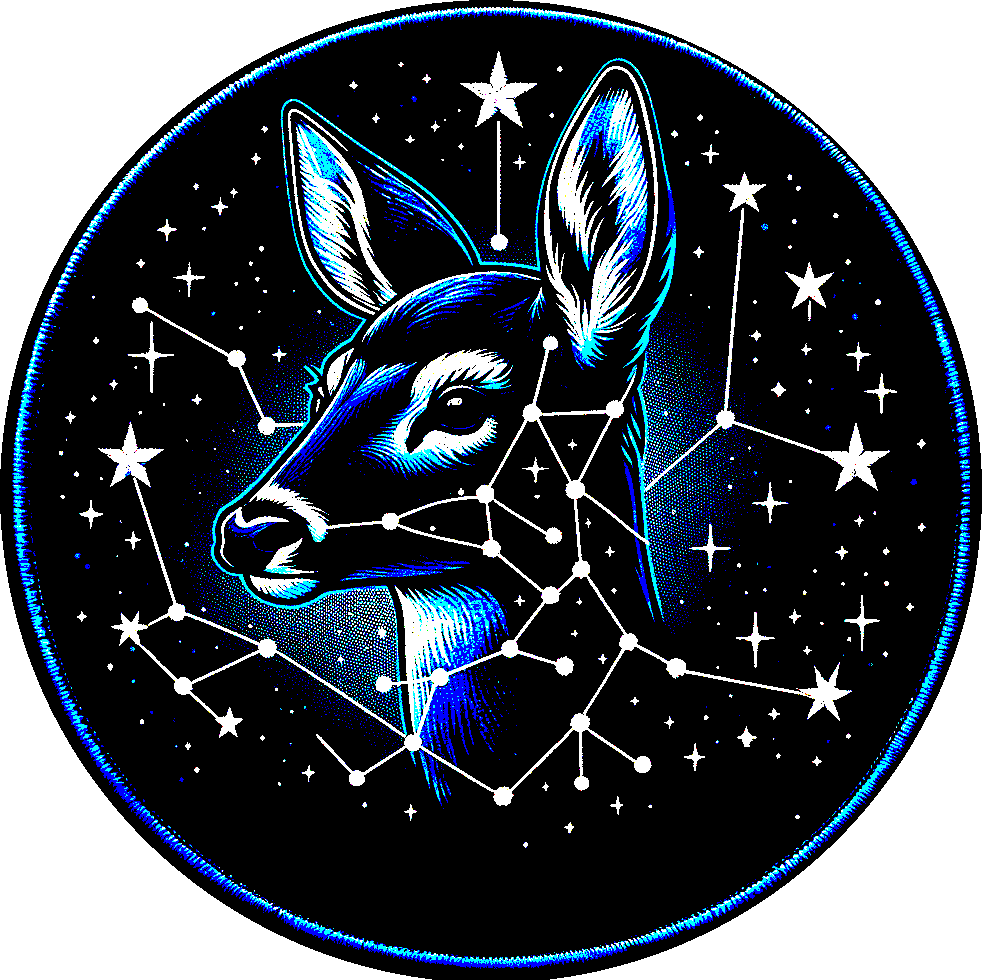
\includegraphics{croppedPosterized.png}};
    \begin{scope}[x={(image.south east)},y={(image.north west)}]

      \draw[black,line width=.4cm] (.5,.5) circle (.49);

      \path[decorate, decoration={
          text along path,
          text={|\patchseries\color{docolor}\fontsize{20pt}{18pt}\selectfont|D~O~E~N~e~t~~~~ L~E~A~P},
          %text={|\patchseries\color{white}\fontsize{60pt}{50pt}\selectfont|XIMERA},
          text align=center
      }] (.02,.5) arc (180:360:.48);








        
      \path[decorate, decoration={
          text along path,
          text={|\patchseries\color{docolor}\fontsize{11pt}{10pt}\selectfont|Distributed Open Education Network~~~~Learning through Exploration and Active Participation},
          text align=center
      }] (.5,.05) arc (270:-90:.45);

      %% \path[decorate, decoration={
      %%     text along path,
      %%     text={|\patchseries\color{white}\fontsize{30pt}{36pt}\selectfont|https://www.github.com/XimeraProject},
      %%     text align=center
      %% }] (.5,.95) arc (90:-40:.45);
      
      %% %\draw[blue] (.5,.95) arc (90:0:.45);




      %% \path[decorate, decoration={
      %%     text along path,
      %%     text={|\patchseries\color{white}\fontsize{30pt}{36pt}\selectfont|https://ximera.osu.edu/mooculus},
      %%     text align=center
      %% }] (.11,.28) arc (210:90:.45);%(.05,.5) arc (210:90:.45);
      
      
      
      %\node[white] at ({.44*cos(235)+.5},{.44*sin(235)+.5}) {\rotatebox{-35}{\qrcode[height=1in]{https://ximera.osu.edu/mooculus}}};
      
      
      %\node[white] at ({.44*cos(305)+.5},{.44*sin(305)+.5}) {\rotatebox{35}{\qrcode[height=1in]{https://www.github.com/XimeraProject}}};

      
      
    \end{scope}
\end{tikzpicture}
\end{document}

\begin{tikzpicture}

\end{tikzpicture}
